\PassOptionsToPackage{unicode=true}{hyperref} % options for packages loaded elsewhere
\PassOptionsToPackage{hyphens}{url}
%
\documentclass[]{book}
\usepackage{lmodern}
\usepackage{amssymb,amsmath}
\usepackage{ifxetex,ifluatex}
\usepackage{fixltx2e} % provides \textsubscript
\ifnum 0\ifxetex 1\fi\ifluatex 1\fi=0 % if pdftex
  \usepackage[T1]{fontenc}
  \usepackage[utf8]{inputenc}
  \usepackage{textcomp} % provides euro and other symbols
\else % if luatex or xelatex
  \usepackage{unicode-math}
  \defaultfontfeatures{Ligatures=TeX,Scale=MatchLowercase}
\fi
% use upquote if available, for straight quotes in verbatim environments
\IfFileExists{upquote.sty}{\usepackage{upquote}}{}
% use microtype if available
\IfFileExists{microtype.sty}{%
\usepackage[]{microtype}
\UseMicrotypeSet[protrusion]{basicmath} % disable protrusion for tt fonts
}{}
\IfFileExists{parskip.sty}{%
\usepackage{parskip}
}{% else
\setlength{\parindent}{0pt}
\setlength{\parskip}{6pt plus 2pt minus 1pt}
}
\usepackage{hyperref}
\hypersetup{
            pdftitle={Supplemental Material: Base Diagnostics},
            pdfauthor={Jose Guadalupe Hernandez},
            pdfborder={0 0 0},
            breaklinks=true}
\urlstyle{same}  % don't use monospace font for urls
\usepackage[margin=1in]{geometry}
\usepackage{color}
\usepackage{fancyvrb}
\newcommand{\VerbBar}{|}
\newcommand{\VERB}{\Verb[commandchars=\\\{\}]}
\DefineVerbatimEnvironment{Highlighting}{Verbatim}{commandchars=\\\{\}}
% Add ',fontsize=\small' for more characters per line
\usepackage{framed}
\definecolor{shadecolor}{RGB}{248,248,248}
\newenvironment{Shaded}{\begin{snugshade}}{\end{snugshade}}
\newcommand{\AlertTok}[1]{\textcolor[rgb]{0.94,0.16,0.16}{#1}}
\newcommand{\AnnotationTok}[1]{\textcolor[rgb]{0.56,0.35,0.01}{\textbf{\textit{#1}}}}
\newcommand{\AttributeTok}[1]{\textcolor[rgb]{0.77,0.63,0.00}{#1}}
\newcommand{\BaseNTok}[1]{\textcolor[rgb]{0.00,0.00,0.81}{#1}}
\newcommand{\BuiltInTok}[1]{#1}
\newcommand{\CharTok}[1]{\textcolor[rgb]{0.31,0.60,0.02}{#1}}
\newcommand{\CommentTok}[1]{\textcolor[rgb]{0.56,0.35,0.01}{\textit{#1}}}
\newcommand{\CommentVarTok}[1]{\textcolor[rgb]{0.56,0.35,0.01}{\textbf{\textit{#1}}}}
\newcommand{\ConstantTok}[1]{\textcolor[rgb]{0.00,0.00,0.00}{#1}}
\newcommand{\ControlFlowTok}[1]{\textcolor[rgb]{0.13,0.29,0.53}{\textbf{#1}}}
\newcommand{\DataTypeTok}[1]{\textcolor[rgb]{0.13,0.29,0.53}{#1}}
\newcommand{\DecValTok}[1]{\textcolor[rgb]{0.00,0.00,0.81}{#1}}
\newcommand{\DocumentationTok}[1]{\textcolor[rgb]{0.56,0.35,0.01}{\textbf{\textit{#1}}}}
\newcommand{\ErrorTok}[1]{\textcolor[rgb]{0.64,0.00,0.00}{\textbf{#1}}}
\newcommand{\ExtensionTok}[1]{#1}
\newcommand{\FloatTok}[1]{\textcolor[rgb]{0.00,0.00,0.81}{#1}}
\newcommand{\FunctionTok}[1]{\textcolor[rgb]{0.00,0.00,0.00}{#1}}
\newcommand{\ImportTok}[1]{#1}
\newcommand{\InformationTok}[1]{\textcolor[rgb]{0.56,0.35,0.01}{\textbf{\textit{#1}}}}
\newcommand{\KeywordTok}[1]{\textcolor[rgb]{0.13,0.29,0.53}{\textbf{#1}}}
\newcommand{\NormalTok}[1]{#1}
\newcommand{\OperatorTok}[1]{\textcolor[rgb]{0.81,0.36,0.00}{\textbf{#1}}}
\newcommand{\OtherTok}[1]{\textcolor[rgb]{0.56,0.35,0.01}{#1}}
\newcommand{\PreprocessorTok}[1]{\textcolor[rgb]{0.56,0.35,0.01}{\textit{#1}}}
\newcommand{\RegionMarkerTok}[1]{#1}
\newcommand{\SpecialCharTok}[1]{\textcolor[rgb]{0.00,0.00,0.00}{#1}}
\newcommand{\SpecialStringTok}[1]{\textcolor[rgb]{0.31,0.60,0.02}{#1}}
\newcommand{\StringTok}[1]{\textcolor[rgb]{0.31,0.60,0.02}{#1}}
\newcommand{\VariableTok}[1]{\textcolor[rgb]{0.00,0.00,0.00}{#1}}
\newcommand{\VerbatimStringTok}[1]{\textcolor[rgb]{0.31,0.60,0.02}{#1}}
\newcommand{\WarningTok}[1]{\textcolor[rgb]{0.56,0.35,0.01}{\textbf{\textit{#1}}}}
\usepackage{longtable,booktabs}
% Fix footnotes in tables (requires footnote package)
\IfFileExists{footnote.sty}{\usepackage{footnote}\makesavenoteenv{longtable}}{}
\usepackage{graphicx,grffile}
\makeatletter
\def\maxwidth{\ifdim\Gin@nat@width>\linewidth\linewidth\else\Gin@nat@width\fi}
\def\maxheight{\ifdim\Gin@nat@height>\textheight\textheight\else\Gin@nat@height\fi}
\makeatother
% Scale images if necessary, so that they will not overflow the page
% margins by default, and it is still possible to overwrite the defaults
% using explicit options in \includegraphics[width, height, ...]{}
\setkeys{Gin}{width=\maxwidth,height=\maxheight,keepaspectratio}
\setlength{\emergencystretch}{3em}  % prevent overfull lines
\providecommand{\tightlist}{%
  \setlength{\itemsep}{0pt}\setlength{\parskip}{0pt}}
\setcounter{secnumdepth}{5}
% Redefines (sub)paragraphs to behave more like sections
\ifx\paragraph\undefined\else
\let\oldparagraph\paragraph
\renewcommand{\paragraph}[1]{\oldparagraph{#1}\mbox{}}
\fi
\ifx\subparagraph\undefined\else
\let\oldsubparagraph\subparagraph
\renewcommand{\subparagraph}[1]{\oldsubparagraph{#1}\mbox{}}
\fi

% set default figure placement to htbp
\makeatletter
\def\fps@figure{htbp}
\makeatother

\usepackage[]{natbib}
\bibliographystyle{apalike}

\title{Supplemental Material: Base Diagnostics}
\author{Jose Guadalupe Hernandez}
\date{2023-08-30}

\begin{document}
\maketitle

{
\setcounter{tocdepth}{1}
\tableofcontents
}
\hypertarget{introduction}{%
\chapter{Introduction}\label{introduction}}

This is the supplemental material for experiments breaking down nondominated sorting into its two main components: phenotypic fitness sharing and nondominated front ranking.
We evaluated these components, along with standard nondominated sorting, on the contradictory objectives diagnostic to measure their contribution on the overall effectiveness of nondominated sorting.

\hypertarget{about-our-supplemental-material}{%
\section{About our supplemental material}\label{about-our-supplemental-material}}

This supplemental material is hosted on \href{https://github.com}{GitHub} using GitHub pages.
The source code and configuration files used to generate this supplemental material can be found in \href{https://github.com/jgh9094/ECJ-2023-Suite-Of-Diagnostic-Metrics-For-Characterizing-Selection-Schemes}{this GitHub repository}.
We compiled our data analyses and supplemental documentation into this nifty web-accessible book using \href{https://bookdown.org/}{bookdown}.

Our supplemental material includes the following paper figures and statistics:

\begin{itemize}
\tightlist
\item
  Nondomintaed sorting breakdown (Section \ref{nodominated-sorting-breakdown})
\end{itemize}

\hypertarget{contributing-authors}{%
\section{Contributing authors}\label{contributing-authors}}

\begin{itemize}
\tightlist
\item
  \href{https://jgh9094.github.io/}{Jose Guadalupe Hernandez}
\item
  \href{https://lalejini.com}{Alexander Lalejini}
\item
  \href{http://ofria.com}{Charles Ofria}
\end{itemize}

\hypertarget{computer-setup}{%
\section{Computer Setup}\label{computer-setup}}

These analyses were conducted in the following computing environment:

\begin{Shaded}
\begin{Highlighting}[]
\KeywordTok{print}\NormalTok{(version)}
\end{Highlighting}
\end{Shaded}

\begin{verbatim}
##                _                           
## platform       x86_64-pc-linux-gnu         
## arch           x86_64                      
## os             linux-gnu                   
## system         x86_64, linux-gnu           
## status                                     
## major          4                           
## minor          3.1                         
## year           2023                        
## month          06                          
## day            16                          
## svn rev        84548                       
## language       R                           
## version.string R version 4.3.1 (2023-06-16)
## nickname       Beagle Scouts
\end{verbatim}

\hypertarget{experimental-setup}{%
\section{Experimental setup}\label{experimental-setup}}

Setting up required variables variables.

\begin{Shaded}
\begin{Highlighting}[]
\CommentTok{# libraries we are using}
\KeywordTok{library}\NormalTok{(ggplot2)}
\KeywordTok{library}\NormalTok{(cowplot)}
\KeywordTok{library}\NormalTok{(dplyr)}
\end{Highlighting}
\end{Shaded}

\begin{verbatim}
## 
## Attaching package: 'dplyr'
\end{verbatim}

\begin{verbatim}
## The following objects are masked from 'package:stats':
## 
##     filter, lag
\end{verbatim}

\begin{verbatim}
## The following objects are masked from 'package:base':
## 
##     intersect, setdiff, setequal, union
\end{verbatim}

\begin{Shaded}
\begin{Highlighting}[]
\KeywordTok{library}\NormalTok{(PupillometryR)}
\end{Highlighting}
\end{Shaded}

\begin{verbatim}
## Loading required package: rlang
\end{verbatim}

\begin{Shaded}
\begin{Highlighting}[]
\CommentTok{# data diractory for gh-pages}
\NormalTok{DATA_DIR =}\StringTok{ '/opt/ECJ-2023-Suite-Of-Diagnostic-Metrics-For-Characterizing-Selection-Schemes/DATA/CONTRADICTORY_NONDOMINATED/'}

\CommentTok{# data diractory for local testing}
\CommentTok{# DATA_DIR = '~/Desktop/Repositories/ECJ-2023-Suite-Of-Diagnostic-Metrics-For-Characterizing-Selection-Schemes/DATA/CONTRADICTORY_NONDOMINATED/'}

\CommentTok{# graph variables}
\NormalTok{SHAPE =}\StringTok{ }\KeywordTok{c}\NormalTok{(}\DecValTok{5}\NormalTok{,}\DecValTok{3}\NormalTok{,}\DecValTok{1}\NormalTok{)}
\NormalTok{cb_palette <-}\StringTok{ }\KeywordTok{c}\NormalTok{(}\StringTok{'#88CCEE'}\NormalTok{,}\StringTok{'#EE7733'}\NormalTok{,}\StringTok{'#EE3377'}\NormalTok{)}
\NormalTok{p_theme <-}\StringTok{ }\KeywordTok{theme}\NormalTok{(}
  \DataTypeTok{plot.title =} \KeywordTok{element_text}\NormalTok{( }\DataTypeTok{face =} \StringTok{"bold"}\NormalTok{, }\DataTypeTok{size =} \DecValTok{20}\NormalTok{, }\DataTypeTok{hjust=}\FloatTok{0.5}\NormalTok{),}
  \DataTypeTok{panel.border =} \KeywordTok{element_blank}\NormalTok{(),}
  \DataTypeTok{panel.grid.minor =} \KeywordTok{element_blank}\NormalTok{(),}
  \DataTypeTok{legend.title=}\KeywordTok{element_text}\NormalTok{(}\DataTypeTok{size=}\DecValTok{18}\NormalTok{, }\DataTypeTok{hjust =} \FloatTok{0.5}\NormalTok{),}
  \DataTypeTok{legend.text=}\KeywordTok{element_text}\NormalTok{(}\DataTypeTok{size=}\DecValTok{10}\NormalTok{),}
  \DataTypeTok{axis.title =} \KeywordTok{element_text}\NormalTok{(}\DataTypeTok{size=}\DecValTok{18}\NormalTok{),}
  \DataTypeTok{axis.text =} \KeywordTok{element_text}\NormalTok{(}\DataTypeTok{size=}\DecValTok{16}\NormalTok{),}
  \DataTypeTok{legend.position=}\StringTok{"bottom"}\NormalTok{,}
  \DataTypeTok{legend.margin =} \KeywordTok{margin}\NormalTok{(}\DecValTok{0}\NormalTok{, }\DecValTok{0}\NormalTok{, }\DecValTok{0}\NormalTok{, }\DecValTok{0}\NormalTok{),}
  \DataTypeTok{panel.background =} \KeywordTok{element_rect}\NormalTok{(}\DataTypeTok{fill =} \StringTok{"#f1f2f5"}\NormalTok{,}
                                  \DataTypeTok{colour =} \StringTok{"white"}\NormalTok{,}
                                  \DataTypeTok{linewidth =} \FloatTok{0.5}\NormalTok{, }\DataTypeTok{linetype =} \StringTok{"solid"}\NormalTok{)}
\NormalTok{)}


\CommentTok{# default variables}
\NormalTok{DIMENSIONALITY =}\StringTok{ }\DecValTok{100}
\NormalTok{GENERATIONS =}\StringTok{ }\DecValTok{50000}

\CommentTok{# selection scheme related stuff}
\NormalTok{ACRO =}\StringTok{ }\KeywordTok{c}\NormalTok{(}\StringTok{'nds'}\NormalTok{,}\StringTok{'nfr'}\NormalTok{,}\StringTok{'pfs'}\NormalTok{)}
\NormalTok{NAMES =}\StringTok{ }\KeywordTok{c}\NormalTok{(}\StringTok{'Nondominated sorting (nds)'}\NormalTok{,}\StringTok{'Nondominated front ranking (nfr)'}\NormalTok{,}\StringTok{'Phenotypic fitness sharing (pfs)'}\NormalTok{)}
\end{Highlighting}
\end{Shaded}

\hypertarget{nondominated-sorting-breakdown}{%
\chapter{Nondominated sorting breakdown}\label{nondominated-sorting-breakdown}}

For these experiments we break down nondominated sorting into its two main components: phenotypic fitness sharing and nondominated front ranking.
We evaluated these components, along with standard nondominated sorting, on the contradictory objectives diagnostic to measure their contribution on the overall effectiveness of nondominated sorting.
Here we present the results for \textbf{activation gene coverage} and \textbf{satisfactory trait coverage} found by each selection scheme on the contradictory objectives diagnostic.
50 replicates are conducted for each scheme explored.

\hypertarget{data-setup}{%
\section{Data setup}\label{data-setup}}

\begin{Shaded}
\begin{Highlighting}[]
\NormalTok{over_time_df <-}\StringTok{ }\KeywordTok{read.csv}\NormalTok{(}\KeywordTok{paste}\NormalTok{(DATA_DIR,}\StringTok{'over-time.csv'}\NormalTok{, }\DataTypeTok{sep =} \StringTok{""}\NormalTok{, }\DataTypeTok{collapse =} \OtherTok{NULL}\NormalTok{), }\DataTypeTok{header =} \OtherTok{TRUE}\NormalTok{, }\DataTypeTok{stringsAsFactors =} \OtherTok{FALSE}\NormalTok{)}
\NormalTok{over_time_df}\OperatorTok{$}\NormalTok{scheme <-}\StringTok{ }\KeywordTok{factor}\NormalTok{(over_time_df}\OperatorTok{$}\NormalTok{scheme, }\DataTypeTok{levels =}\NormalTok{ NAMES)}
\NormalTok{over_time_df}\OperatorTok{$}\NormalTok{acro <-}\StringTok{ }\KeywordTok{factor}\NormalTok{(over_time_df}\OperatorTok{$}\NormalTok{acro, }\DataTypeTok{levels =}\NormalTok{ ACRO)}
\end{Highlighting}
\end{Shaded}

\hypertarget{activation-gene-coverage-over-time}{%
\section{Activation gene coverage over time}\label{activation-gene-coverage-over-time}}

Activation gene coverage in a population over time.
Data points on the graph is the average activation gene coverage across 50 replicates every 2000 generations.
Shading comes from the best and worse coverage across 50 replicates.

\begin{Shaded}
\begin{Highlighting}[]
\NormalTok{lines =}\StringTok{ }\NormalTok{over_time_df }\OperatorTok
\StringTok{  }\KeywordTok{group_by}\NormalTok{(scheme, gen) }\OperatorTok
\StringTok{  }\NormalTok{dplyr}\OperatorTok{::}\KeywordTok{summarise}\NormalTok{(}
    \DataTypeTok{min =} \KeywordTok{min}\NormalTok{(uni_str_pos),}
    \DataTypeTok{mean =} \KeywordTok{mean}\NormalTok{(uni_str_pos),}
    \DataTypeTok{max =} \KeywordTok{max}\NormalTok{(uni_str_pos)}
\NormalTok{  )}
\end{Highlighting}
\end{Shaded}

\begin{verbatim}
## `summarise()` has grouped output by 'scheme'. You can override using the
## `.groups` argument.
\end{verbatim}

\begin{Shaded}
\begin{Highlighting}[]
\NormalTok{over_time_plot =}\StringTok{ }\KeywordTok{ggplot}\NormalTok{(lines, }\KeywordTok{aes}\NormalTok{(}\DataTypeTok{x=}\NormalTok{gen, }\DataTypeTok{y=}\NormalTok{mean, }\DataTypeTok{group =}\NormalTok{ scheme, }\DataTypeTok{fill =}\NormalTok{ scheme, }\DataTypeTok{color =}\NormalTok{ scheme, }\DataTypeTok{shape =}\NormalTok{ scheme)) }\OperatorTok{+}
\StringTok{  }\KeywordTok{geom_ribbon}\NormalTok{(}\KeywordTok{aes}\NormalTok{(}\DataTypeTok{ymin =}\NormalTok{ min, }\DataTypeTok{ymax =}\NormalTok{ max), }\DataTypeTok{alpha =} \FloatTok{0.1}\NormalTok{) }\OperatorTok{+}
\StringTok{  }\KeywordTok{geom_line}\NormalTok{(}\DataTypeTok{size =} \FloatTok{0.5}\NormalTok{) }\OperatorTok{+}
\StringTok{  }\KeywordTok{geom_point}\NormalTok{(}\DataTypeTok{data =} \KeywordTok{filter}\NormalTok{(lines, gen }\OperatorTok\StringTok{ }\DecValTok{2000} \OperatorTok{==}\StringTok{ }\DecValTok{0} \OperatorTok{&}\StringTok{ }\NormalTok{gen }\OperatorTok{!=}\StringTok{ }\DecValTok{0}\NormalTok{), }\DataTypeTok{size =} \FloatTok{1.5}\NormalTok{, }\DataTypeTok{stroke =} \FloatTok{2.0}\NormalTok{, }\DataTypeTok{alpha =} \FloatTok{1.0}\NormalTok{) }\OperatorTok{+}
\StringTok{  }\KeywordTok{scale_y_continuous}\NormalTok{(}
    \DataTypeTok{name=}\StringTok{"Coverage"}\NormalTok{,}
    \DataTypeTok{limits=}\KeywordTok{c}\NormalTok{(}\DecValTok{0}\NormalTok{, }\DecValTok{100}\NormalTok{),}
    \DataTypeTok{breaks=}\KeywordTok{seq}\NormalTok{(}\DecValTok{0}\NormalTok{,}\DecValTok{100}\NormalTok{, }\DecValTok{20}\NormalTok{),}
    \DataTypeTok{labels=}\KeywordTok{c}\NormalTok{(}\StringTok{"0"}\NormalTok{, }\StringTok{"20"}\NormalTok{, }\StringTok{"40"}\NormalTok{, }\StringTok{"60"}\NormalTok{, }\StringTok{"80"}\NormalTok{, }\StringTok{"100"}\NormalTok{)}
\NormalTok{  ) }\OperatorTok{+}
\StringTok{  }\KeywordTok{scale_x_continuous}\NormalTok{(}
    \DataTypeTok{name=}\StringTok{"Generations"}\NormalTok{,}
    \DataTypeTok{limits=}\KeywordTok{c}\NormalTok{(}\DecValTok{0}\NormalTok{, }\DecValTok{50000}\NormalTok{),}
    \DataTypeTok{breaks=}\KeywordTok{c}\NormalTok{(}\DecValTok{0}\NormalTok{, }\DecValTok{10000}\NormalTok{, }\DecValTok{20000}\NormalTok{, }\DecValTok{30000}\NormalTok{, }\DecValTok{40000}\NormalTok{, }\DecValTok{50000}\NormalTok{),}
    \DataTypeTok{labels=}\KeywordTok{c}\NormalTok{(}\StringTok{"0e+4"}\NormalTok{, }\StringTok{"1e+4"}\NormalTok{, }\StringTok{"2e+4"}\NormalTok{, }\StringTok{"3e+4"}\NormalTok{, }\StringTok{"4e+4"}\NormalTok{, }\StringTok{"5e+4"}\NormalTok{)}
\NormalTok{  ) }\OperatorTok{+}
\StringTok{  }\KeywordTok{scale_shape_manual}\NormalTok{(}\DataTypeTok{values=}\NormalTok{SHAPE)}\OperatorTok{+}
\StringTok{  }\KeywordTok{scale_colour_manual}\NormalTok{(}\DataTypeTok{values =}\NormalTok{ cb_palette) }\OperatorTok{+}
\StringTok{  }\KeywordTok{scale_fill_manual}\NormalTok{(}\DataTypeTok{values =}\NormalTok{ cb_palette) }\OperatorTok{+}
\StringTok{  }\KeywordTok{ggtitle}\NormalTok{(}\StringTok{'Activation gene coverage over time'}\NormalTok{)}\OperatorTok{+}
\StringTok{  }\NormalTok{p_theme }\OperatorTok{+}
\StringTok{  }\KeywordTok{guides}\NormalTok{(}
    \DataTypeTok{shape=}\KeywordTok{guide_legend}\NormalTok{(}\DataTypeTok{ncol=}\DecValTok{1}\NormalTok{, }\DataTypeTok{title.position =} \StringTok{"left"}\NormalTok{, }\DataTypeTok{title =} \StringTok{'Selection }\CharTok{\textbackslash{}n}\StringTok{Scheme'}\NormalTok{),}
    \DataTypeTok{color=}\KeywordTok{guide_legend}\NormalTok{(}\DataTypeTok{ncol=}\DecValTok{1}\NormalTok{, }\DataTypeTok{title.position =} \StringTok{"left"}\NormalTok{, }\DataTypeTok{title =} \StringTok{'Selection }\CharTok{\textbackslash{}n}\StringTok{Scheme'}\NormalTok{),}
    \DataTypeTok{fill=}\KeywordTok{guide_legend}\NormalTok{(}\DataTypeTok{ncol=}\DecValTok{1}\NormalTok{, }\DataTypeTok{title.position =} \StringTok{"left"}\NormalTok{, }\DataTypeTok{title =} \StringTok{'Selection }\CharTok{\textbackslash{}n}\StringTok{Scheme'}\NormalTok{)}
\NormalTok{  )}
\NormalTok{over_time_plot}
\end{Highlighting}
\end{Shaded}

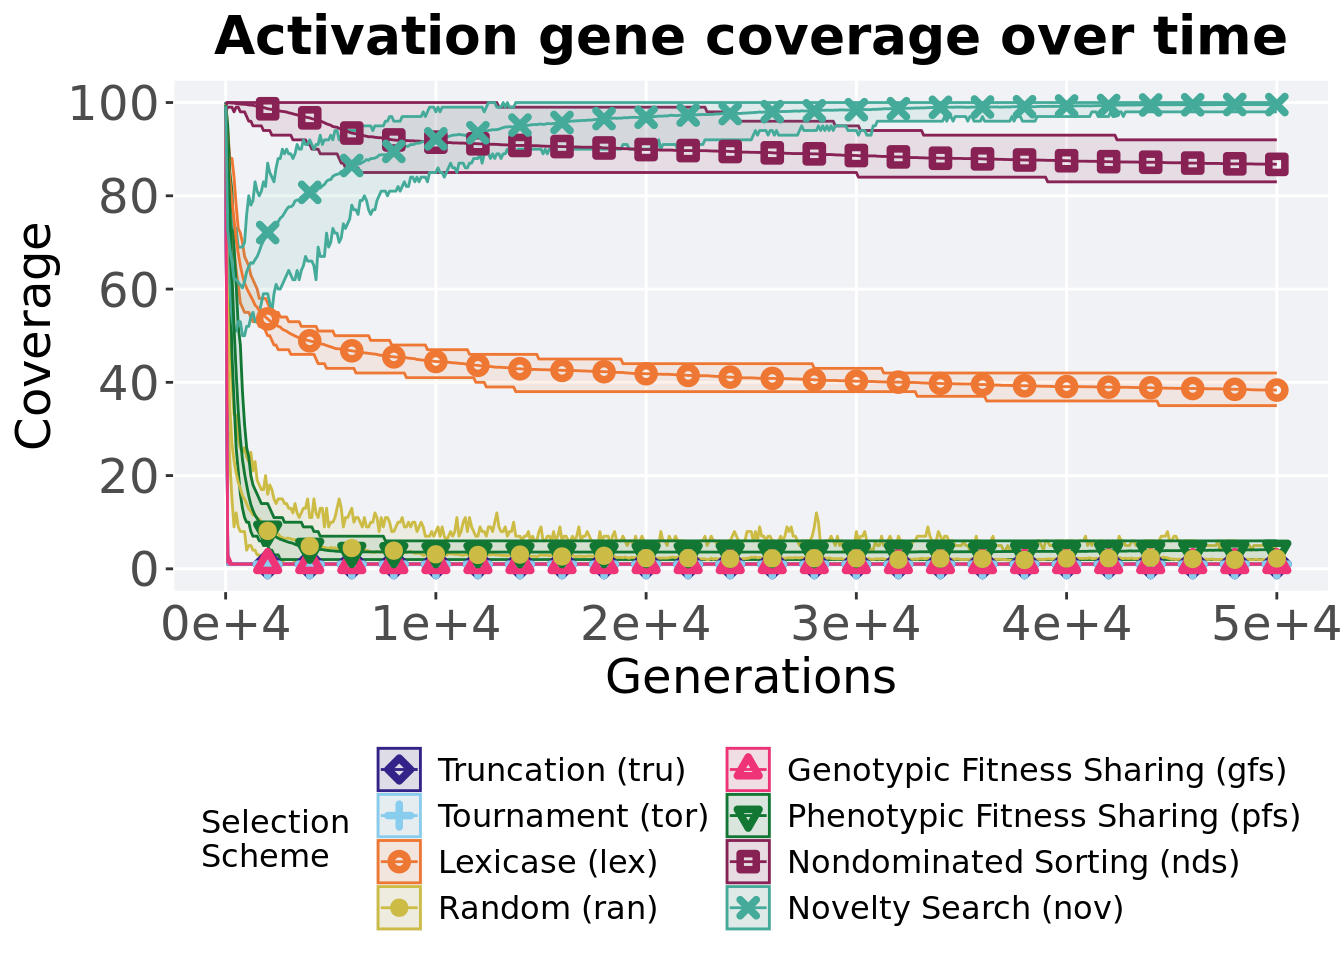
\includegraphics[width=1\linewidth]{contradictory-nondominated-sorting-breakdown_files/figure-latex/con-act-ot-1}

\hypertarget{final-activation-gene-coverage}{%
\section{Final activation gene coverage}\label{final-activation-gene-coverage}}

Activation gene coverage found in the final population at 50,000 generations.

\begin{Shaded}
\begin{Highlighting}[]
\NormalTok{plot =}\StringTok{ }\KeywordTok{filter}\NormalTok{(over_time_df, gen }\OperatorTok{==}\StringTok{ }\DecValTok{50000}\NormalTok{) }\OperatorTok
\StringTok{  }\KeywordTok{ggplot}\NormalTok{(., }\KeywordTok{aes}\NormalTok{(}\DataTypeTok{x =}\NormalTok{ acro, }\DataTypeTok{y =}\NormalTok{ uni_str_pos, }\DataTypeTok{color =}\NormalTok{ acro, }\DataTypeTok{fill =}\NormalTok{ acro, }\DataTypeTok{shape =}\NormalTok{ acro)) }\OperatorTok{+}
\StringTok{  }\KeywordTok{geom_flat_violin}\NormalTok{(}\DataTypeTok{position =} \KeywordTok{position_nudge}\NormalTok{(}\DataTypeTok{x =} \FloatTok{.1}\NormalTok{, }\DataTypeTok{y =} \DecValTok{0}\NormalTok{), }\DataTypeTok{scale =} \StringTok{'width'}\NormalTok{, }\DataTypeTok{alpha =} \FloatTok{0.2}\NormalTok{, }\DataTypeTok{width =} \FloatTok{1.5}\NormalTok{) }\OperatorTok{+}
\StringTok{  }\KeywordTok{geom_boxplot}\NormalTok{(}\DataTypeTok{color =} \StringTok{'black'}\NormalTok{, }\DataTypeTok{width =} \FloatTok{.07}\NormalTok{, }\DataTypeTok{outlier.shape =} \OtherTok{NA}\NormalTok{, }\DataTypeTok{alpha =} \FloatTok{0.0}\NormalTok{, }\DataTypeTok{size =} \FloatTok{1.0}\NormalTok{, }\DataTypeTok{position =} \KeywordTok{position_nudge}\NormalTok{(}\DataTypeTok{x =} \FloatTok{.16}\NormalTok{, }\DataTypeTok{y =} \DecValTok{0}\NormalTok{)) }\OperatorTok{+}
\StringTok{  }\KeywordTok{geom_point}\NormalTok{(}\DataTypeTok{position =} \KeywordTok{position_jitter}\NormalTok{(}\DataTypeTok{width =} \FloatTok{0.03}\NormalTok{, }\DataTypeTok{height =} \FloatTok{0.02}\NormalTok{), }\DataTypeTok{size =} \FloatTok{2.0}\NormalTok{, }\DataTypeTok{alpha =} \FloatTok{1.0}\NormalTok{) }\OperatorTok{+}
\StringTok{  }\KeywordTok{scale_y_continuous}\NormalTok{(}
    \DataTypeTok{name=}\StringTok{"Coverage"}\NormalTok{,}
    \DataTypeTok{limits=}\KeywordTok{c}\NormalTok{(}\DecValTok{0}\NormalTok{, }\DecValTok{100}\NormalTok{),}
    \DataTypeTok{breaks=}\KeywordTok{seq}\NormalTok{(}\DecValTok{0}\NormalTok{,}\DecValTok{100}\NormalTok{, }\DecValTok{20}\NormalTok{),}
    \DataTypeTok{labels=}\KeywordTok{c}\NormalTok{(}\StringTok{"0"}\NormalTok{, }\StringTok{"20"}\NormalTok{, }\StringTok{"40"}\NormalTok{, }\StringTok{"60"}\NormalTok{, }\StringTok{"80"}\NormalTok{, }\StringTok{"100"}\NormalTok{)}
\NormalTok{  ) }\OperatorTok{+}
\StringTok{  }\KeywordTok{scale_x_discrete}\NormalTok{(}
    \DataTypeTok{name=}\StringTok{"Scheme"}
\NormalTok{  )}\OperatorTok{+}
\StringTok{  }\KeywordTok{scale_shape_manual}\NormalTok{(}\DataTypeTok{values=}\NormalTok{SHAPE)}\OperatorTok{+}
\StringTok{  }\KeywordTok{scale_colour_manual}\NormalTok{(}\DataTypeTok{values =}\NormalTok{ cb_palette, ) }\OperatorTok{+}
\StringTok{  }\KeywordTok{scale_fill_manual}\NormalTok{(}\DataTypeTok{values =}\NormalTok{ cb_palette) }\OperatorTok{+}
\StringTok{  }\KeywordTok{ggtitle}\NormalTok{(}\StringTok{'Final activation gene coverage'}\NormalTok{)}\OperatorTok{+}
\StringTok{  }\NormalTok{p_theme}

\KeywordTok{plot_grid}\NormalTok{(}
\NormalTok{  plot }\OperatorTok{+}
\StringTok{    }\KeywordTok{theme}\NormalTok{(}\DataTypeTok{legend.position=}\StringTok{"none"}\NormalTok{),}
\NormalTok{  legend,}
  \DataTypeTok{nrow=}\DecValTok{2}\NormalTok{,}
  \DataTypeTok{rel_heights =} \KeywordTok{c}\NormalTok{(}\DecValTok{3}\NormalTok{,}\DecValTok{1}\NormalTok{)}
\NormalTok{)}
\end{Highlighting}
\end{Shaded}

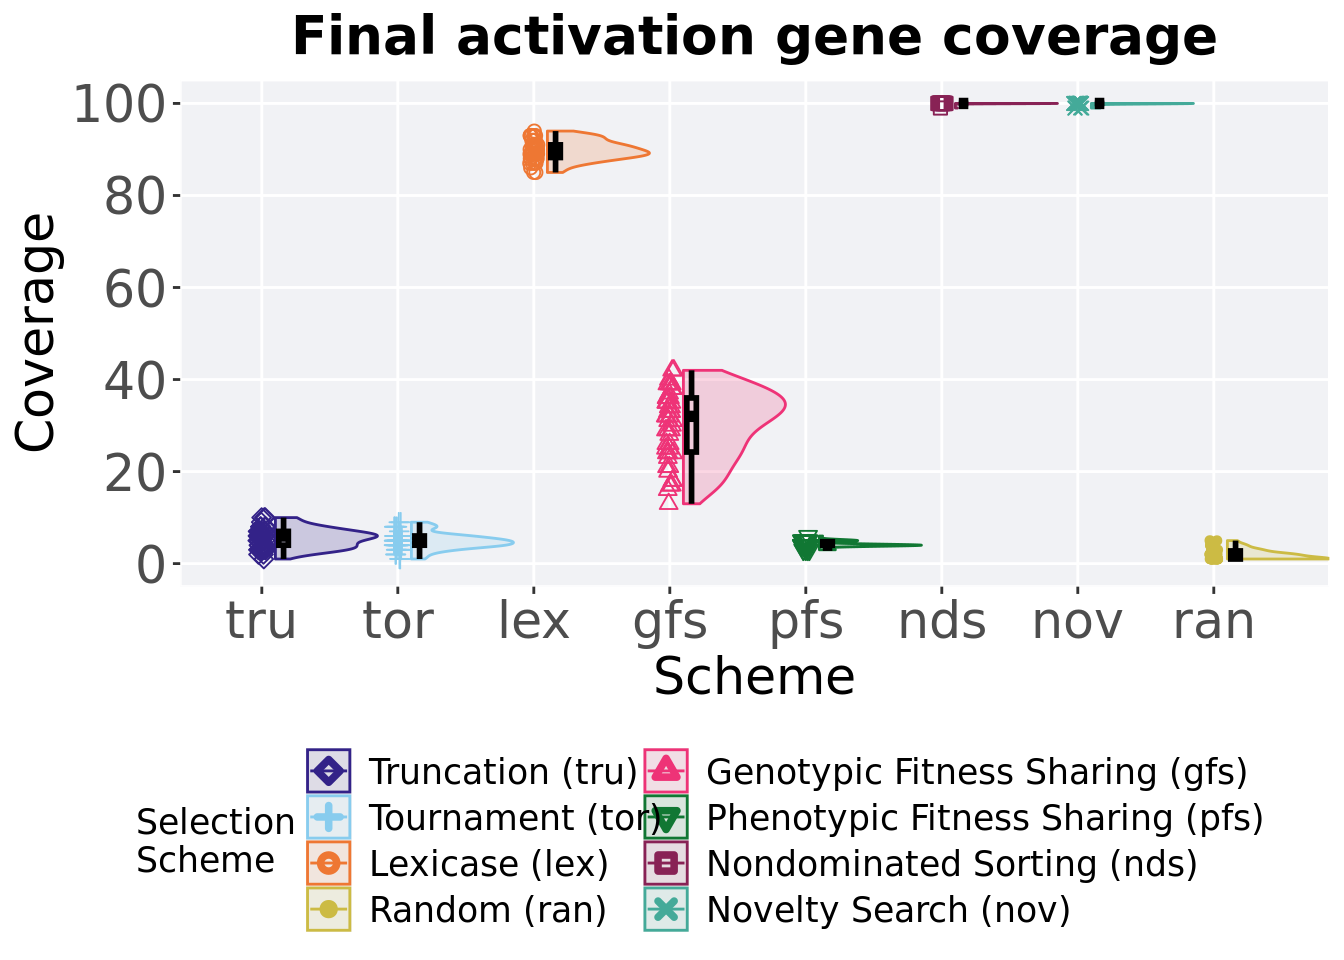
\includegraphics[width=1\linewidth]{contradictory-nondominated-sorting-breakdown_files/figure-latex/con-act-end-1}

\hypertarget{stats}{%
\subsection{Stats}\label{stats}}

Summary statistics for the coverage found in the final population.

\begin{Shaded}
\begin{Highlighting}[]
\NormalTok{act_coverage =}\StringTok{ }\KeywordTok{filter}\NormalTok{(over_time_df, gen }\OperatorTok{==}\StringTok{ }\DecValTok{50000}\NormalTok{)}
\NormalTok{act_coverage}\OperatorTok{$}\NormalTok{acro =}\StringTok{ }\KeywordTok{factor}\NormalTok{(act_coverage}\OperatorTok{$}\NormalTok{acro, }\DataTypeTok{levels =} \KeywordTok{c}\NormalTok{(}\StringTok{'nds'}\NormalTok{,}\StringTok{'pfs'}\NormalTok{,}\StringTok{'nfr'}\NormalTok{))}
\NormalTok{act_coverage }\OperatorTok
\StringTok{  }\KeywordTok{group_by}\NormalTok{(acro) }\OperatorTok
\StringTok{  }\NormalTok{dplyr}\OperatorTok{::}\KeywordTok{summarise}\NormalTok{(}
    \DataTypeTok{count =} \KeywordTok{n}\NormalTok{(),}
    \DataTypeTok{na_cnt =} \KeywordTok{sum}\NormalTok{(}\KeywordTok{is.na}\NormalTok{(uni_str_pos)),}
    \DataTypeTok{min =} \KeywordTok{min}\NormalTok{(uni_str_pos, }\DataTypeTok{na.rm =} \OtherTok{TRUE}\NormalTok{),}
    \DataTypeTok{median =} \KeywordTok{median}\NormalTok{(uni_str_pos, }\DataTypeTok{na.rm =} \OtherTok{TRUE}\NormalTok{),}
    \DataTypeTok{mean =} \KeywordTok{mean}\NormalTok{(uni_str_pos, }\DataTypeTok{na.rm =} \OtherTok{TRUE}\NormalTok{),}
    \DataTypeTok{max =} \KeywordTok{max}\NormalTok{(uni_str_pos, }\DataTypeTok{na.rm =} \OtherTok{TRUE}\NormalTok{),}
    \DataTypeTok{IQR =} \KeywordTok{IQR}\NormalTok{(uni_str_pos, }\DataTypeTok{na.rm =} \OtherTok{TRUE}\NormalTok{)}
\NormalTok{  )}
\end{Highlighting}
\end{Shaded}

\begin{verbatim}
## # A tibble: 3 x 8
##   acro  count na_cnt   min median  mean   max   IQR
##   <fct> <int>  <int> <int>  <dbl> <dbl> <int> <dbl>
## 1 nds      50      0    84     87 86.8     91  2.75
## 2 pfs      50      0     3      4  4.04     6  2   
## 3 nfr      50      0     1      1  1.44     3  1
\end{verbatim}

Kruskal--Wallis test illustrates evidence of statistical differences.

\begin{Shaded}
\begin{Highlighting}[]
\KeywordTok{kruskal.test}\NormalTok{(uni_str_pos }\OperatorTok{~}\StringTok{ }\NormalTok{acro, }\DataTypeTok{data =}\NormalTok{ act_coverage)}
\end{Highlighting}
\end{Shaded}

\begin{verbatim}
## 
##  Kruskal-Wallis rank sum test
## 
## data:  uni_str_pos by acro
## Kruskal-Wallis chi-squared = 133.91, df = 2, p-value < 2.2e-16
\end{verbatim}

Results for post-hoc Wilcoxon rank-sum test with a Bonferroni correction.

\begin{Shaded}
\begin{Highlighting}[]
\KeywordTok{pairwise.wilcox.test}\NormalTok{(}\DataTypeTok{x =}\NormalTok{ act_coverage}\OperatorTok{$}\NormalTok{uni_str_pos, }\DataTypeTok{g =}\NormalTok{ act_coverage}\OperatorTok{$}\NormalTok{acro, }\DataTypeTok{p.adjust.method =} \StringTok{"bonferroni"}\NormalTok{,}
                     \DataTypeTok{paired =} \OtherTok{FALSE}\NormalTok{, }\DataTypeTok{conf.int =} \OtherTok{FALSE}\NormalTok{, }\DataTypeTok{alternative =} \StringTok{'l'}\NormalTok{)}
\end{Highlighting}
\end{Shaded}

\begin{verbatim}
## 
##  Pairwise comparisons using Wilcoxon rank sum test with continuity correction 
## 
## data:  act_coverage$uni_str_pos and act_coverage$acro 
## 
##     nds    pfs   
## pfs <2e-16 -     
## nfr <2e-16 <2e-16
## 
## P value adjustment method: bonferroni
\end{verbatim}

\hypertarget{satisfactory-trait-coverage-over-time}{%
\section{Satisfactory trait coverage over time}\label{satisfactory-trait-coverage-over-time}}

Satisfactory trait coverage in a population over time.
Data points on the graph is the average activation gene coverage across 50 replicates every 2000 generations.
Shading comes from the best and worse coverage across 50 replicates.

\begin{Shaded}
\begin{Highlighting}[]
\NormalTok{lines =}\StringTok{ }\NormalTok{over_time_df }\OperatorTok
\StringTok{  }\KeywordTok{group_by}\NormalTok{(scheme, gen) }\OperatorTok
\StringTok{  }\NormalTok{dplyr}\OperatorTok{::}\KeywordTok{summarise}\NormalTok{(}
    \DataTypeTok{min =} \KeywordTok{min}\NormalTok{(pop_uni_obj),}
    \DataTypeTok{mean =} \KeywordTok{mean}\NormalTok{(pop_uni_obj),}
    \DataTypeTok{max =} \KeywordTok{max}\NormalTok{(pop_uni_obj)}
\NormalTok{  )}
\end{Highlighting}
\end{Shaded}

\begin{verbatim}
## `summarise()` has grouped output by 'scheme'. You can override using the
## `.groups` argument.
\end{verbatim}

\begin{Shaded}
\begin{Highlighting}[]
\NormalTok{over_time_plot =}\StringTok{ }\KeywordTok{ggplot}\NormalTok{(lines, }\KeywordTok{aes}\NormalTok{(}\DataTypeTok{x=}\NormalTok{gen, }\DataTypeTok{y=}\NormalTok{mean, }\DataTypeTok{group =}\NormalTok{ scheme, }\DataTypeTok{fill =}\NormalTok{ scheme, }\DataTypeTok{color =}\NormalTok{ scheme, }\DataTypeTok{shape =}\NormalTok{ scheme)) }\OperatorTok{+}
\StringTok{  }\KeywordTok{geom_ribbon}\NormalTok{(}\KeywordTok{aes}\NormalTok{(}\DataTypeTok{ymin =}\NormalTok{ min, }\DataTypeTok{ymax =}\NormalTok{ max), }\DataTypeTok{alpha =} \FloatTok{0.1}\NormalTok{) }\OperatorTok{+}
\StringTok{  }\KeywordTok{geom_line}\NormalTok{(}\DataTypeTok{size =} \FloatTok{0.5}\NormalTok{) }\OperatorTok{+}
\StringTok{  }\KeywordTok{geom_point}\NormalTok{(}\DataTypeTok{data =} \KeywordTok{filter}\NormalTok{(lines, gen }\OperatorTok\StringTok{ }\DecValTok{2000} \OperatorTok{==}\StringTok{ }\DecValTok{0} \OperatorTok{&}\StringTok{ }\NormalTok{gen }\OperatorTok{!=}\StringTok{ }\DecValTok{0}\NormalTok{), }\DataTypeTok{size =} \FloatTok{1.5}\NormalTok{, }\DataTypeTok{stroke =} \FloatTok{2.0}\NormalTok{, }\DataTypeTok{alpha =} \FloatTok{1.0}\NormalTok{) }\OperatorTok{+}
\StringTok{  }\KeywordTok{scale_y_continuous}\NormalTok{(}
    \DataTypeTok{name=}\StringTok{"Coverage"}\NormalTok{,}
    \DataTypeTok{limits=}\KeywordTok{c}\NormalTok{(}\DecValTok{0}\NormalTok{, }\DecValTok{100}\NormalTok{),}
    \DataTypeTok{breaks=}\KeywordTok{seq}\NormalTok{(}\DecValTok{0}\NormalTok{,}\DecValTok{100}\NormalTok{, }\DecValTok{20}\NormalTok{),}
    \DataTypeTok{labels=}\KeywordTok{c}\NormalTok{(}\StringTok{"0"}\NormalTok{, }\StringTok{"20"}\NormalTok{, }\StringTok{"40"}\NormalTok{, }\StringTok{"60"}\NormalTok{, }\StringTok{"80"}\NormalTok{, }\StringTok{"100"}\NormalTok{)}
\NormalTok{  ) }\OperatorTok{+}
\StringTok{  }\KeywordTok{scale_x_continuous}\NormalTok{(}
    \DataTypeTok{name=}\StringTok{"Generations"}\NormalTok{,}
    \DataTypeTok{limits=}\KeywordTok{c}\NormalTok{(}\DecValTok{0}\NormalTok{, }\DecValTok{50000}\NormalTok{),}
    \DataTypeTok{breaks=}\KeywordTok{c}\NormalTok{(}\DecValTok{0}\NormalTok{, }\DecValTok{10000}\NormalTok{, }\DecValTok{20000}\NormalTok{, }\DecValTok{30000}\NormalTok{, }\DecValTok{40000}\NormalTok{, }\DecValTok{50000}\NormalTok{),}
    \DataTypeTok{labels=}\KeywordTok{c}\NormalTok{(}\StringTok{"0e+4"}\NormalTok{, }\StringTok{"1e+4"}\NormalTok{, }\StringTok{"2e+4"}\NormalTok{, }\StringTok{"3e+4"}\NormalTok{, }\StringTok{"4e+4"}\NormalTok{, }\StringTok{"5e+4"}\NormalTok{)}

\NormalTok{  ) }\OperatorTok{+}
\StringTok{  }\KeywordTok{scale_shape_manual}\NormalTok{(}\DataTypeTok{values=}\NormalTok{SHAPE)}\OperatorTok{+}
\StringTok{  }\KeywordTok{scale_colour_manual}\NormalTok{(}\DataTypeTok{values =}\NormalTok{ cb_palette) }\OperatorTok{+}
\StringTok{  }\KeywordTok{scale_fill_manual}\NormalTok{(}\DataTypeTok{values =}\NormalTok{ cb_palette) }\OperatorTok{+}
\StringTok{  }\KeywordTok{ggtitle}\NormalTok{(}\StringTok{'Satisfactory trait coverage over time'}\NormalTok{)}\OperatorTok{+}
\StringTok{  }\NormalTok{p_theme }\OperatorTok{+}
\StringTok{  }\KeywordTok{guides}\NormalTok{(}
    \DataTypeTok{shape=}\KeywordTok{guide_legend}\NormalTok{(}\DataTypeTok{ncol=}\DecValTok{1}\NormalTok{, }\DataTypeTok{title.position =} \StringTok{"left"}\NormalTok{, }\DataTypeTok{title =} \StringTok{'Selection }\CharTok{\textbackslash{}n}\StringTok{Scheme'}\NormalTok{),}
    \DataTypeTok{color=}\KeywordTok{guide_legend}\NormalTok{(}\DataTypeTok{ncol=}\DecValTok{1}\NormalTok{, }\DataTypeTok{title.position =} \StringTok{"left"}\NormalTok{, }\DataTypeTok{title =} \StringTok{'Selection }\CharTok{\textbackslash{}n}\StringTok{Scheme'}\NormalTok{),}
    \DataTypeTok{fill=}\KeywordTok{guide_legend}\NormalTok{(}\DataTypeTok{ncol=}\DecValTok{1}\NormalTok{, }\DataTypeTok{title.position =} \StringTok{"left"}\NormalTok{, }\DataTypeTok{title =} \StringTok{'Selection }\CharTok{\textbackslash{}n}\StringTok{Scheme'}\NormalTok{)}
\NormalTok{  )}
\end{Highlighting}
\end{Shaded}

\hypertarget{final-satisfactory-trait-coverage}{%
\section{Final satisfactory trait coverage}\label{final-satisfactory-trait-coverage}}

Satisfactory trait coverage found in the final population at 50,000 generations.

\begin{Shaded}
\begin{Highlighting}[]
\NormalTok{plot =}\StringTok{ }\KeywordTok{filter}\NormalTok{(over_time_df, gen }\OperatorTok{==}\StringTok{ }\DecValTok{50000}\NormalTok{) }\OperatorTok
\StringTok{  }\KeywordTok{ggplot}\NormalTok{(., }\KeywordTok{aes}\NormalTok{(}\DataTypeTok{x =}\NormalTok{ acro, }\DataTypeTok{y =}\NormalTok{ pop_uni_obj, }\DataTypeTok{color =}\NormalTok{ acro, }\DataTypeTok{fill =}\NormalTok{ acro, }\DataTypeTok{shape =}\NormalTok{ acro)) }\OperatorTok{+}
\StringTok{  }\KeywordTok{geom_flat_violin}\NormalTok{(}\DataTypeTok{position =} \KeywordTok{position_nudge}\NormalTok{(}\DataTypeTok{x =} \FloatTok{.1}\NormalTok{, }\DataTypeTok{y =} \DecValTok{0}\NormalTok{), }\DataTypeTok{scale =} \StringTok{'width'}\NormalTok{, }\DataTypeTok{alpha =} \FloatTok{0.2}\NormalTok{, }\DataTypeTok{width =} \FloatTok{1.5}\NormalTok{) }\OperatorTok{+}
\StringTok{  }\KeywordTok{geom_boxplot}\NormalTok{(}\DataTypeTok{color =} \StringTok{'black'}\NormalTok{, }\DataTypeTok{width =} \FloatTok{.07}\NormalTok{, }\DataTypeTok{outlier.shape =} \OtherTok{NA}\NormalTok{, }\DataTypeTok{alpha =} \FloatTok{0.0}\NormalTok{, }\DataTypeTok{size =} \FloatTok{1.0}\NormalTok{, }\DataTypeTok{position =} \KeywordTok{position_nudge}\NormalTok{(}\DataTypeTok{x =} \FloatTok{.16}\NormalTok{, }\DataTypeTok{y =} \DecValTok{0}\NormalTok{)) }\OperatorTok{+}
\StringTok{  }\KeywordTok{geom_point}\NormalTok{(}\DataTypeTok{position =} \KeywordTok{position_jitter}\NormalTok{(}\DataTypeTok{width =} \FloatTok{0.03}\NormalTok{, }\DataTypeTok{height =} \FloatTok{0.02}\NormalTok{), }\DataTypeTok{size =} \FloatTok{2.0}\NormalTok{, }\DataTypeTok{alpha =} \FloatTok{1.0}\NormalTok{) }\OperatorTok{+}
\StringTok{  }\KeywordTok{scale_y_continuous}\NormalTok{(}
    \DataTypeTok{name=}\StringTok{"Coverage"}\NormalTok{,}
    \DataTypeTok{limits=}\KeywordTok{c}\NormalTok{(}\DecValTok{0}\NormalTok{, }\DecValTok{100}\NormalTok{),}
    \DataTypeTok{breaks=}\KeywordTok{seq}\NormalTok{(}\DecValTok{0}\NormalTok{,}\DecValTok{100}\NormalTok{, }\DecValTok{20}\NormalTok{),}
    \DataTypeTok{labels=}\KeywordTok{c}\NormalTok{(}\StringTok{"0"}\NormalTok{, }\StringTok{"20"}\NormalTok{, }\StringTok{"40"}\NormalTok{, }\StringTok{"60"}\NormalTok{, }\StringTok{"80"}\NormalTok{, }\StringTok{"100"}\NormalTok{)}
\NormalTok{  ) }\OperatorTok{+}
\StringTok{  }\KeywordTok{scale_x_discrete}\NormalTok{(}
    \DataTypeTok{name=}\StringTok{"Scheme"}
\NormalTok{  )}\OperatorTok{+}
\StringTok{  }\KeywordTok{scale_shape_manual}\NormalTok{(}\DataTypeTok{values=}\NormalTok{SHAPE)}\OperatorTok{+}
\StringTok{  }\KeywordTok{scale_colour_manual}\NormalTok{(}\DataTypeTok{values =}\NormalTok{ cb_palette, ) }\OperatorTok{+}
\StringTok{  }\KeywordTok{scale_fill_manual}\NormalTok{(}\DataTypeTok{values =}\NormalTok{ cb_palette) }\OperatorTok{+}
\StringTok{  }\KeywordTok{ggtitle}\NormalTok{(}\StringTok{'Final satisfactory trait coverage'}\NormalTok{)}\OperatorTok{+}
\StringTok{  }\NormalTok{p_theme}

\KeywordTok{plot_grid}\NormalTok{(}
\NormalTok{  plot }\OperatorTok{+}
\StringTok{    }\KeywordTok{theme}\NormalTok{(}\DataTypeTok{legend.position=}\StringTok{"none"}\NormalTok{),}
\NormalTok{  legend,}
  \DataTypeTok{nrow=}\DecValTok{2}\NormalTok{,}
  \DataTypeTok{rel_heights =} \KeywordTok{c}\NormalTok{(}\DecValTok{3}\NormalTok{,}\DecValTok{1}\NormalTok{)}
\NormalTok{)}
\end{Highlighting}
\end{Shaded}

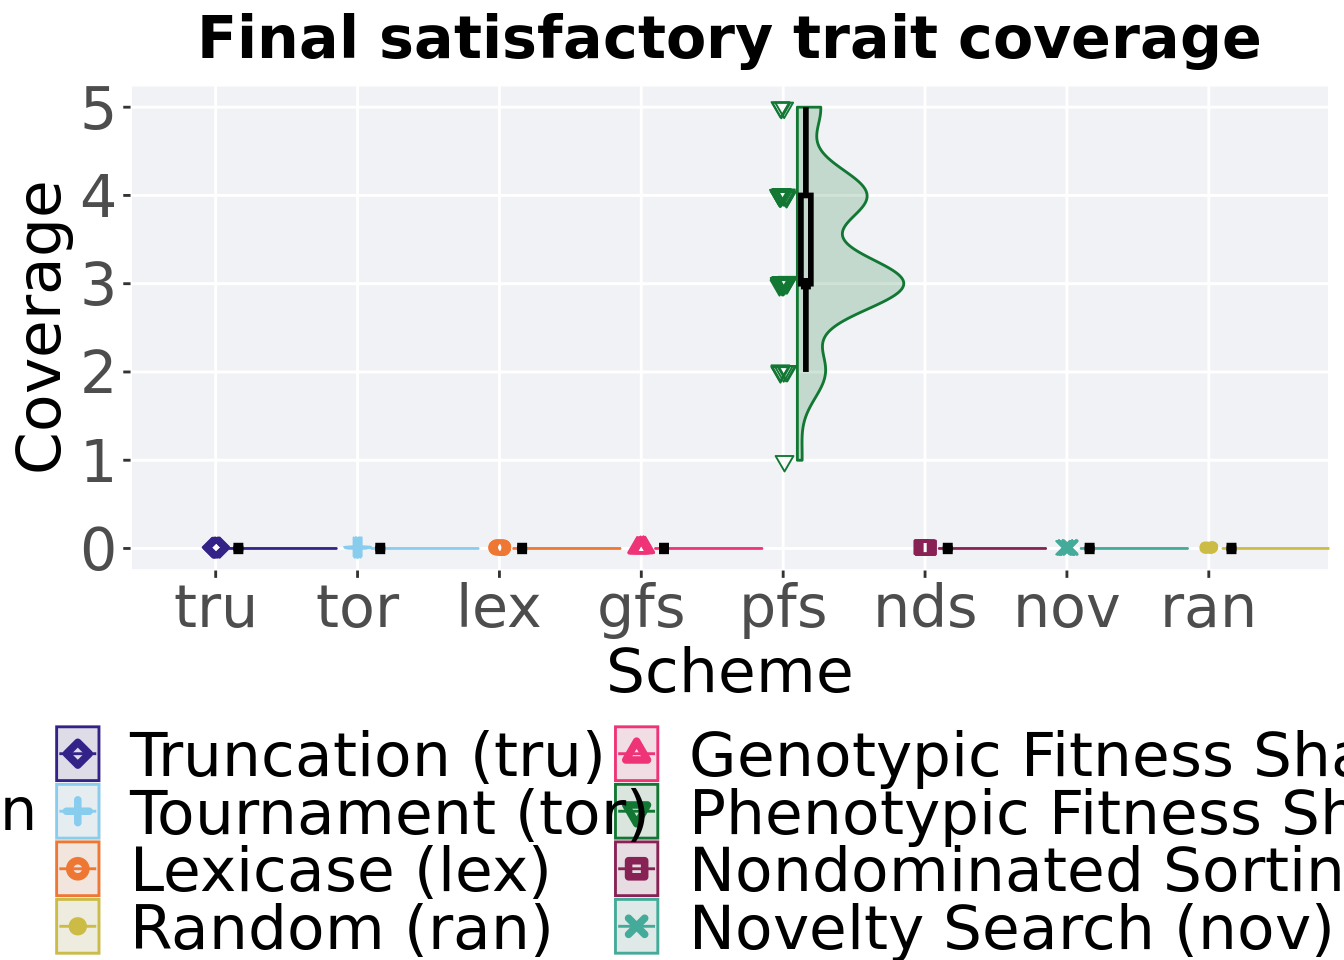
\includegraphics[width=1\linewidth]{contradictory-nondominated-sorting-breakdown_files/figure-latex/con-sat-end-1}

\hypertarget{stats-1}{%
\subsection{Stats}\label{stats-1}}

Summary statistics for the coverage found in the final population.

\begin{Shaded}
\begin{Highlighting}[]
\NormalTok{sat_coverage =}\StringTok{ }\KeywordTok{filter}\NormalTok{(over_time_df, gen }\OperatorTok{==}\StringTok{ }\DecValTok{50000}\NormalTok{)}
\NormalTok{sat_coverage}\OperatorTok{$}\NormalTok{acro =}\StringTok{ }\KeywordTok{factor}\NormalTok{(sat_coverage}\OperatorTok{$}\NormalTok{acro, }\DataTypeTok{levels =} \KeywordTok{c}\NormalTok{(}\StringTok{'nds'}\NormalTok{,}\StringTok{'pfs'}\NormalTok{,}\StringTok{'nfr'}\NormalTok{))}
\NormalTok{sat_coverage }\OperatorTok
\StringTok{  }\KeywordTok{group_by}\NormalTok{(acro) }\OperatorTok
\StringTok{  }\NormalTok{dplyr}\OperatorTok{::}\KeywordTok{summarise}\NormalTok{(}
    \DataTypeTok{count =} \KeywordTok{n}\NormalTok{(),}
    \DataTypeTok{na_cnt =} \KeywordTok{sum}\NormalTok{(}\KeywordTok{is.na}\NormalTok{(pop_uni_obj)),}
    \DataTypeTok{min =} \KeywordTok{min}\NormalTok{(pop_uni_obj, }\DataTypeTok{na.rm =} \OtherTok{TRUE}\NormalTok{),}
    \DataTypeTok{median =} \KeywordTok{median}\NormalTok{(pop_uni_obj, }\DataTypeTok{na.rm =} \OtherTok{TRUE}\NormalTok{),}
    \DataTypeTok{mean =} \KeywordTok{mean}\NormalTok{(pop_uni_obj, }\DataTypeTok{na.rm =} \OtherTok{TRUE}\NormalTok{),}
    \DataTypeTok{max =} \KeywordTok{max}\NormalTok{(pop_uni_obj, }\DataTypeTok{na.rm =} \OtherTok{TRUE}\NormalTok{),}
    \DataTypeTok{IQR =} \KeywordTok{IQR}\NormalTok{(pop_uni_obj, }\DataTypeTok{na.rm =} \OtherTok{TRUE}\NormalTok{)}
\NormalTok{  )}
\end{Highlighting}
\end{Shaded}

\begin{verbatim}
## # A tibble: 3 x 8
##   acro  count na_cnt   min median  mean   max   IQR
##   <fct> <int>  <int> <int>  <dbl> <dbl> <int> <dbl>
## 1 nds      50      0    84     87 86.8     91  2.75
## 2 pfs      50      0     3      4  3.86     6  1   
## 3 nfr      50      0     1      1  1.4      3  1
\end{verbatim}

Kruskal--Wallis test illustrates evidence of statistical differences.

\begin{Shaded}
\begin{Highlighting}[]
\KeywordTok{kruskal.test}\NormalTok{(pop_uni_obj }\OperatorTok{~}\StringTok{ }\NormalTok{acro, }\DataTypeTok{data =}\NormalTok{ sat_coverage)}
\end{Highlighting}
\end{Shaded}

\begin{verbatim}
## 
##  Kruskal-Wallis rank sum test
## 
## data:  pop_uni_obj by acro
## Kruskal-Wallis chi-squared = 134.12, df = 2, p-value < 2.2e-16
\end{verbatim}

Results for post-hoc Wilcoxon rank-sum test with a Bonferroni correction.

\begin{Shaded}
\begin{Highlighting}[]
\KeywordTok{pairwise.wilcox.test}\NormalTok{(}\DataTypeTok{x =}\NormalTok{ sat_coverage}\OperatorTok{$}\NormalTok{pop_uni_obj, }\DataTypeTok{g =}\NormalTok{ sat_coverage}\OperatorTok{$}\NormalTok{acro, }\DataTypeTok{p.adjust.method =} \StringTok{"bonferroni"}\NormalTok{,}
                     \DataTypeTok{paired =} \OtherTok{FALSE}\NormalTok{, }\DataTypeTok{conf.int =} \OtherTok{FALSE}\NormalTok{, }\DataTypeTok{alternative =} \StringTok{'l'}\NormalTok{)}
\end{Highlighting}
\end{Shaded}

\begin{verbatim}
## 
##  Pairwise comparisons using Wilcoxon rank sum test with continuity correction 
## 
## data:  sat_coverage$pop_uni_obj and sat_coverage$acro 
## 
##     nds    pfs   
## pfs <2e-16 -     
## nfr <2e-16 <2e-16
## 
## P value adjustment method: bonferroni
\end{verbatim}

\end{document}
